\section{Funktionen}

Die App Collector soll den folgenden Beschriebenen Funktionsumfang besitzen. Dieser wurde anhand der Recherche, der Ist-Analyse und dem Bedarf von M. Weigert ermittelt. Probleme bei der Umsetzung der Funktionen und deshalb nötige Anpassungen werden im Kapitel \ref{ch:Umsetzung} ab Seite \pageref{ch:Umsetzung} dokumentiert.

\newpage

\begin{landscape}
	\section{Übersicht Funktionen}
	\label{sec:UebersichtFunktion}
	\begin{figure}[htbp]
		\centering
		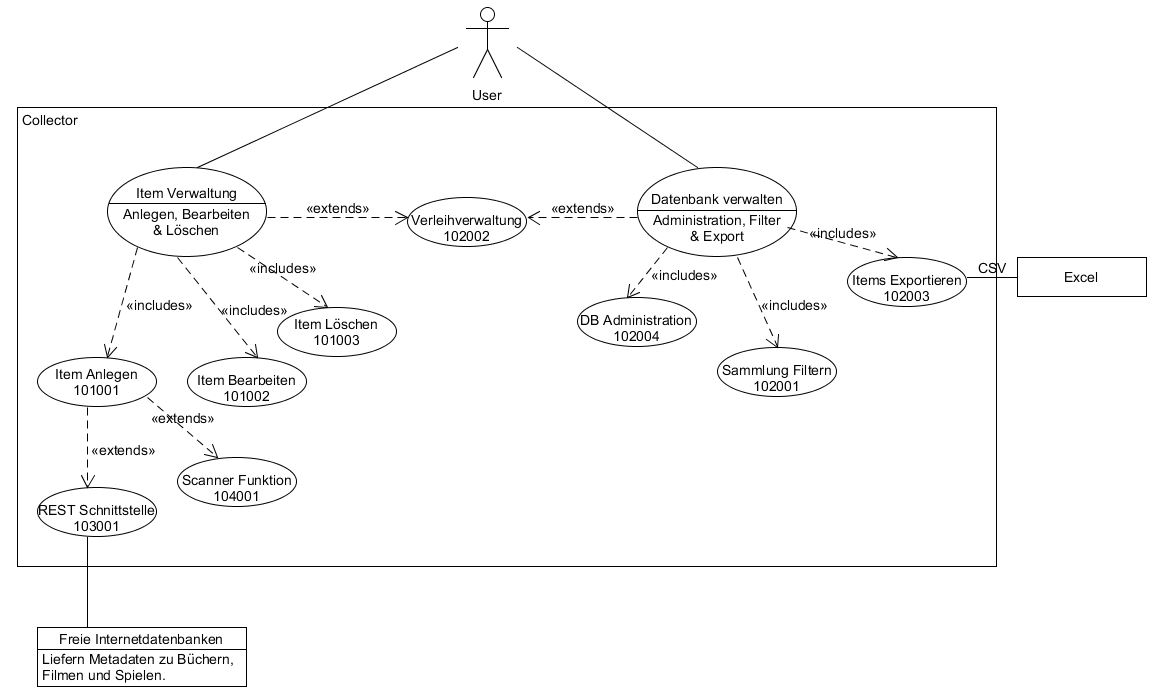
\includegraphics[scale=0.65]{pic/SystemUseCase}
		\caption{Überblick Funktionen}
	\end{figure}
\end{landscape}

\subsection{Anlegen eines Items}

[101001] Funktion: Item Anlegen\\

Das Anlegen eines neuen Items soll auf zweierlei Arten Möglich sein.

\begin{enumerate}
	\item Manuell
	\item Automatisch
\end{enumerate}

Nach der Auswahl {\color{IndianRed}\texttt{Neues Item}} wird standardmässig der Screen für das automatische Anlegen eines Items, mit aktivierter Kamera, geöffnet. Auf diesem Screen gibt es einen Button für das manuelle Anlegen eines Items.

\subsubsection{Manuelles Anlegen eines Items}

Sobald der User {\color{IndianRed}\texttt{manuell}} ausgewählt hat öffnet sich der Screen für Bearbeiten und Manuelles anlegen eines Items. Da es sich hierbei um die neu Anlage eines Items handelt ist der Screen noch komplett ohne angezeigte Daten.\\

Nun kann der User alle Parameter, welche ein Item besitzt manuell eingeben und speichern. Um welche Daten es sich hierbei handelt ist in diesem Kapitel im Absatz \ref{sec:Felder} ab Seite \pageref{sec:Felder} dokumentiert.

\begin{figure}[htbp]
	\centering
	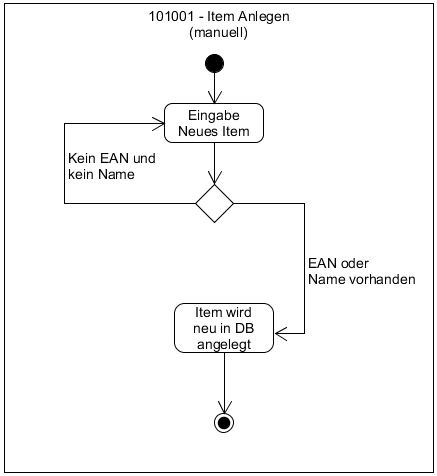
\includegraphics[scale=0.6]{pic/101001m}
	\caption{Aktivitätsdiagramm: Manuell Item anlegen}
\end{figure}

\subsubsection{Automatisches Anlegen eines Items}

Das automatische Anlegen eines Items ist in der App als Standard, für das Anlegen eines Items definiert. Sobald der User {\color{IndianRed}\texttt{Neues Item}} ausgewählt hat öffnet sich die Kamera. Der User muss nun nur noch den Barcode scannen (photographieren) und eine automatische Suche, im Internet, nach Metadaten zu diesem Barcode wird gestartet. Die gefundenen Metadaten werden dem User angezeigt und er kann diese nun bestätigen oder noch anpassen.

\begin{figure}[htbp]
	\centering
	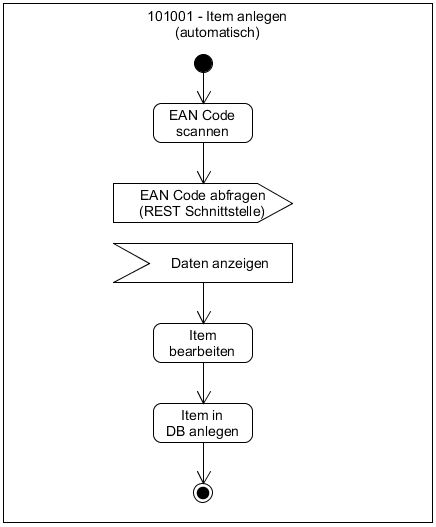
\includegraphics[scale=0.6]{pic/101001a}
	\caption{Aktivitätsdiagramm: Automatisch Item anlegen}
\end{figure}

\subsection{Bearbeiten eines Items}

[101002] Funktion: Item Bearbeiten\\

Ein vom User ausgewähltes Item, kann durch die Funktion {\color{IndianRed}\texttt{Bearbeiten}} manuell bearbeitet werden. Es gibt für den User keine Einschränkungen, jedes Datenelement kann angepasst werden.

\begin{figure}[htbp]
	\centering
	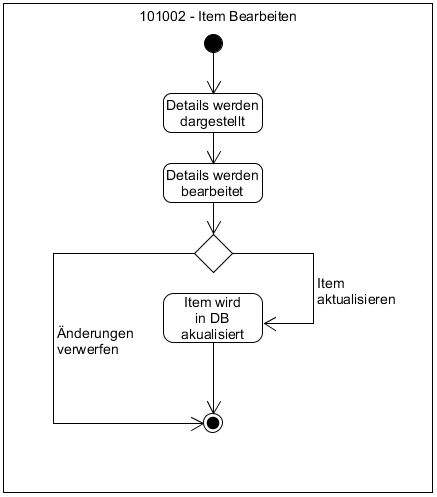
\includegraphics[scale=0.6]{pic/101002}
	\caption{Aktivitätsdiagramm: Item bearbeiten}
\end{figure}

\subsection{Löschen eines Items}

[101003] Funktion: Item löschen\\

Ein vom User ausgewähltes Item, wird komplett (mit all seinen Datenelementen) und unwiderruflich aus der Datenbank gelöscht. Zum Schutz vor unfreiwilligem Löschen, wird vor dem durchführen der Löschung der User nochmals aufgefordert den Löschvorgang zu bestätigen.

\begin{figure}[htbp]
	\centering
	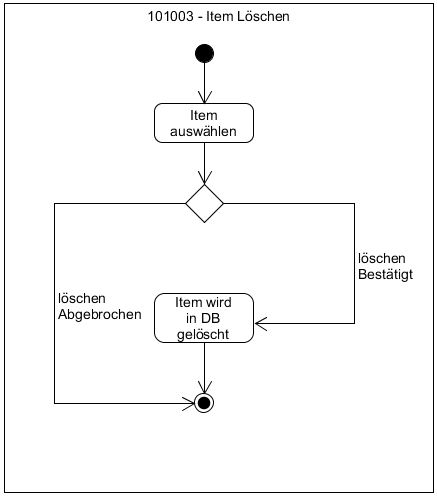
\includegraphics[scale=0.6]{pic/101003}
	\caption{Aktivitätsdiagramm: Item löschen}
\end{figure}

\subsection{Ausgabe der Items}

[102001] Funktion: Items anzeigen\\

Der User kann sich entweder die komplette Sammlung anzeigen lassen oder durch Eingabe eines oder mehreren Filterkriterien die angezeigt Auswahl einschränken. Jedes Kriterium, welches von einem Item gespeichert wird kann als Filter verwendet werden. Werden vom User mehrere Kriterien angegeben, werden diese mittels einer \emph{UND Verknüpfung} im Filter verwendet. 

\begin{figure}[htbp]
	\centering
	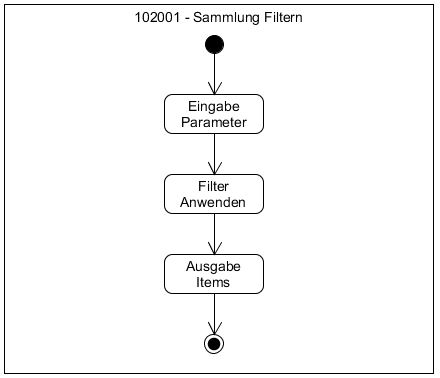
\includegraphics[scale=0.6]{pic/102001}
	\caption{Aktivitätsdiagramm: Sammlung anzeigen}
\end{figure}

\subsection{Verwalten verliehener Items}

[102002] Funktion: Items anzeigen\\

Der User kann ein Item als verliehen markieren. Wird ein Item so markiert, wird der User aufgefordert die leihende Person und das Datum einzugeben. Bei der Rückgabe des Items wird der Status von verliehen auf nicht verliehen geändert und das Item erscheint nun nicht mehr auf der Liste der verliehenen Gegenständen.\\
Eine History zeigt alle jemals verliehenen Gegenstände an.

\begin{figure}[htbp]
	\centering
	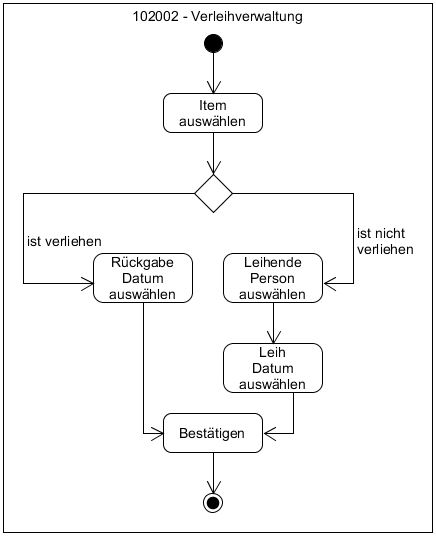
\includegraphics[scale=0.6]{pic/102002}
	\caption{Aktivitätsdiagramm: Verwalten verliehener Items}
\end{figure}

\subsection{Exportieren aller ausgewählter Items}

[102003] Funktion: Items anzeigen\\

Eine vollständige oder gefilterte Übersicht der Items einer Sammlung kann als CSV File exportiert werden. Das Export File wird auf der Speicherkarte des Smartphones gespeichert. Zusätzlich wird ein Mailprogramm geöffnet mittels welchem man das Export File versenden kann.

\begin{figure}[htbp]
	\centering
	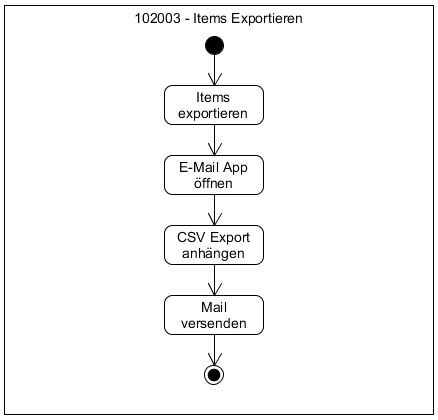
\includegraphics[scale=0.6]{pic/102003}
	\caption{Aktivitätsdiagramm: Export der Sammlung}
\end{figure}

\subsection{Datenbank Administration}

[102004] Funktion: Datenbank Administration\\

Die Datenbank Administration unterstützt folgende drei Aktionen für alle vorhanden Tables.

\begin{enumerate}
	\item Hinzufügen eines Eintrages
	\item Entfernen eines Eintrages
	\item Löschen der ausgewählten Tabelle
\end{enumerate}

\begin{figure}[htbp]
	\centering
	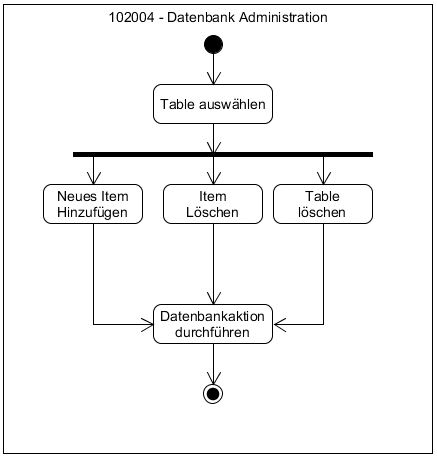
\includegraphics[scale=0.6]{pic/102004}
	\caption{Aktivitätsdiagramm: Datenbank Administration}
\end{figure}

\subsection{REST Schnittstelle zur Abfrage von Metadaten diverser Online Datenbanken}

[103001] Funktion: REST Schnittstelle zur Abfrage von Metadaten\\

Über eine REST Schnittstelle soll die App verschiedene Online Datenbanken abfragen. Anhand des gesendeten EAN Codes sollen eventuell vorhandene Metadaten zu den Items erfragt werden, so damit der User nicht alle Daten von Hand eingeben muss.

\subsection{Kamera als Barcodescanner}

[104001] Funktion: Kamera als Barcodescanner\\

Als weitere Eingabehilfe für den User soll die Kamera des Smartphones als EAN Scanner genutzt werden. Sollte diese den Barcode nicht erkennen können, kann der Barcode vom User manuell eingegeben werden.
